\documentclass[12pt]{article}

\usepackage[top=3.5cm, bottom=3cm, left=2.5cm , right=2.5cm]{geometry}

\usepackage[utf8]{inputenc}
\usepackage[T1]{fontenc}
\usepackage{hyperref}
\usepackage{amsfonts}
\usepackage{amsmath}
\usepackage{amssymb}
\usepackage{setspace}
\usepackage{fancyhdr}
\usepackage{lipsum}
\usepackage{graphicx}
\usepackage[german=guillemets]{csquotes}
\usepackage{lmodern,blindtext}
\DeclareGraphicsExtensions{.pdf,.png,.jpg}

\newcommand{\Matiere}{Génie des Logiciels et des Systèmes}
\newcommand{\titre}{Modélisation, Vérification et Génération de Jeux}

\title{\Matiere:\\ \titre}
\author{Kévin CARENOU \and Thibault MEUNIER \and Matthieu PERRIER \and Sacha VANLEENE}
\date{15 décembre 2016}

\pagestyle{fancy}
\fancyhead[L]{\titre}
\fancyhead[R]{\nouppercase{\leftmark}}
\fancyfoot[L]{\Matiere}
\fancyfoot[C]{Page \thepage}
\fancyfoot[R]{ENSEEIHT - IMA 2A}

\begin{document}
\maketitle

\setcounter{page}{0}
\thispagestyle{empty} % enlever numerotation de la page de garde

\newpage

\section*{Introdution}
Ce projet a pour objectif de modeliser un jeu via un langage propre, de s'assurer de sa faisabilite par un mecanisme de verification automatique et d'offrir la possibilite d'y jouer. 
\newline

Il s'agit d'un outil desirant simplifier le travail de son utilisateur. Lorsque celui-ci concoit le jeu de demain, il est aide par une syntaxe simple, des mecanismes de verification, une execution rapide dans une interface dediee. C'est pourquoi  chaque etape du developpement a ete pensee pour etre utilisable sans friction.
\newline
Plusieurs jeux de demonstrations ont ainsi ete crees afin de confronter nos idees a leur mise en pratique. Par soucis de simplicite, ce rapport ne retiendra que l'exemple du jeu d'enigme decrit ci-dessous.
\textquote{Le territoire est composé de trois lieux, un de début nommé Enigme et  deux  de  fin  qui  représentent  le  succès,  nommé Succès, et  l’échec, Echec.  Ces trois lieux sont qualifiés par leur nom. Le nombre de réponses possibles est représenté par un objet Tentative dont l’explorateur possède un nombre initial, par exemple 3. Le lieu Enigme contient une personne Sphinx qui est visible et obligatoire. Cette personne est qualifiée par le texte de la question. Son interaction contient un choix dont chaque action est qualifiée par les réponses possibles. L’action associée aux mauvaises réponses consomme un objet Tentative. L’action associée aux bonnes réponses donne une connaissance Réussite. Il existe un chemin obligatoire allant du lieu Enigme au lieu Succès dont la visibilité est conditionnée par la possession de la connaissance Réussite. Il existe un chemin obligatoire allant du lieu Enigme au lieu Echec dont la visibilité est conditionnée par la possession d’un nombre d’objet Tentative égal à 0.}
\newline

Le projet s'est revele ambitieux et le present rapport s'attache a en montrer une version simplifiee mais fonctionelle. Les divers choix que nous avons ete amenes a prendre seront detailles et explique. Les documents presentes sont le fruit d'une reflexion commune au membre du groupe et le resultat de dialogues repetes.
\newpage

\renewcommand{\contentsname}{Sommaire}
\tableofcontents
\newpage

\section{Syntaxe Textuelle}
\subsection{Langage Game}
Pour modeliser son jeu, l'utilisateur devait disposer d'une syntaxe textuelle simple. Le choix d'un langage s'approchant d'une description naturelle nous a semble une bonne reponse a ce probleme. En limitant le nombre de mot cle et en laissant beaucoup de parametres facultatifs, l'utilisateur beneficie d'une grande liberte dans la realisation de son jeu. Les declarations s'eloigne d'une description ordonnee des donnees au profit d'instantiations masquees. Nous avons egalement eu le soucis de la factorisation du code en ne faisant pas repete a l'utilisateur des informations identiques. Ceci est gere par la creation dynamique de lien.
\newline\newline
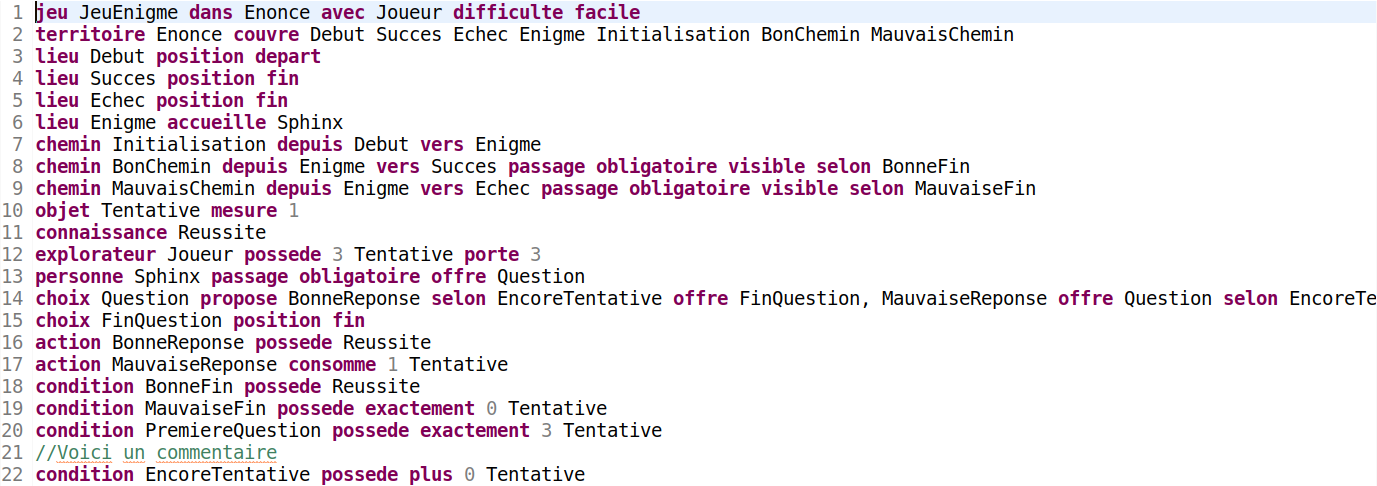
\includegraphics[width=\textwidth]{images/enigme_game}
\newline\newline
Un application directe de cette creation a la volee est les objets. L'utilisateur declare simplement un objet simple (ici Tentative) et un objet comprenant la quantite est cree a chaque fois que celui-ci est utilise (avec 3 Tentative par exemple, le modele cree un objet "3 Tentative") sans declaration explicite.\newline
On note egalement la possibilite d'effectuer des commentaires. Ceux-ci sont egalement accessible au travers du modele decrit ci-apres. Il serait donc possible de permettre a un utilisateur avance d'agir sur la generation du code par l'intermediaire de macro (semblable a la JavaDoc).
Les fichiers de declaration de jeu seront enregistres au format ".game".

\subsection{Metamodele et contraintes statiques}
L'interet d'utiliser Xtext est de beneficier des outils de generation de modele. Les fichiers modeles seront regroupes sous l'extension ".gamemodel". Notre interet s'etant focalise sur la simplicite du langage, le modele genere est assez complexe et nous allons donc detaille seulement les parties principales.\newline
Le jeu se presente de la facon suivante:
\newline\newline
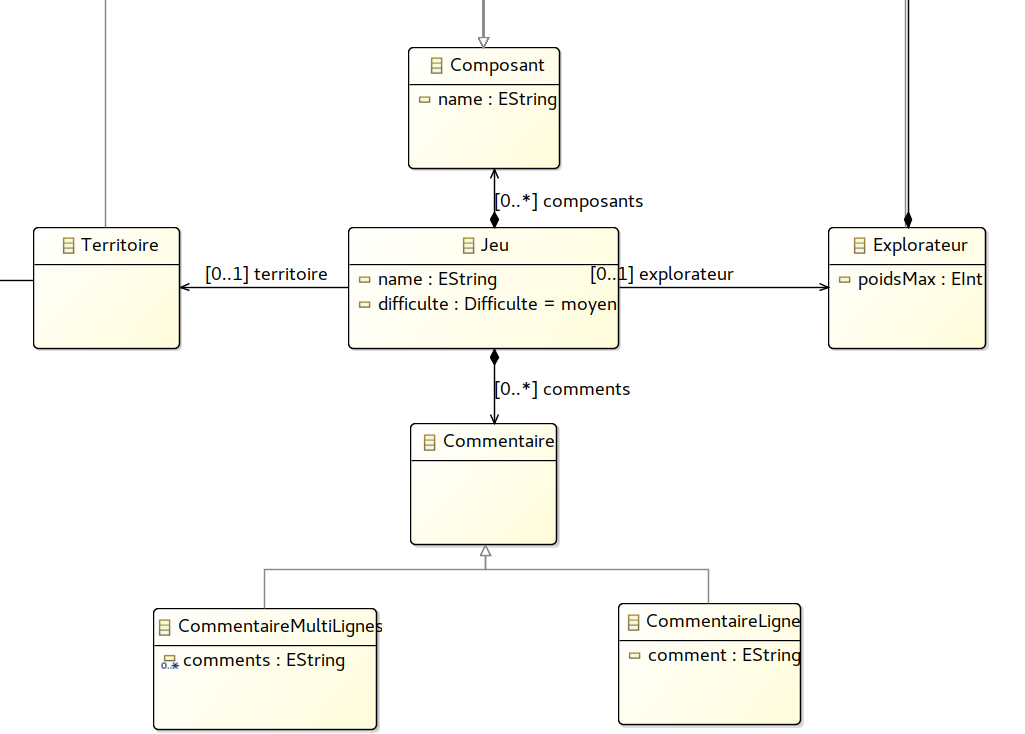
\includegraphics[width=\textwidth]{images/diagram_Jeu}
\newline\newline
Les composants sont les objets declares explicitement par l'utilisateur. Il y a autant de composant que de declaration dans le fichier du jeu. Ils presentent tous un nom permettant de les identifies. Les objets dont l'instanciations est masquee ne sont pas considere comme des composants et on un identifiant unique genere par Xtext. Notons au passage que le territoire et l'explorateur sont des composants. Plusieurs peuvent avoir ete declares mais un seul de chaque sera lie au jeu.\newline
\newline
L'un des points essentiels est l'absence de boolean dans le modele. Nous leur avons prefere l'emploi d'enumeration, plus explicite et modulable. Une relation binaire de prime abord peut se devoiler etre plus complexe et necessite la definition d'un troisieme etat.
\newline\newline
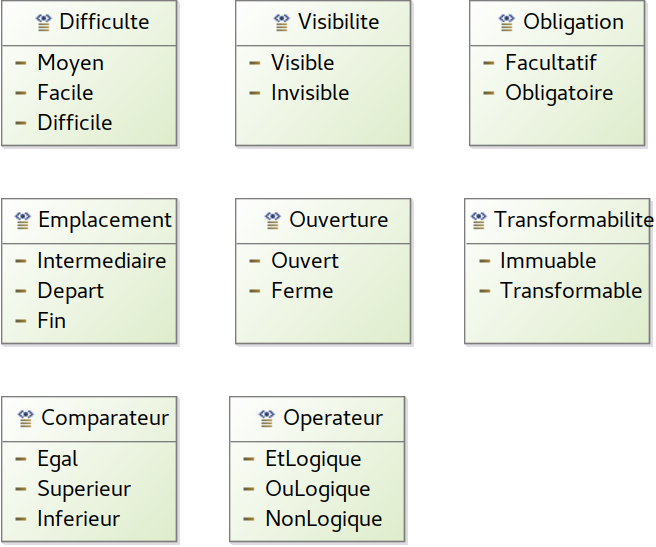
\includegraphics[width=\textwidth]{images/diagram_Enums}
\newline\newline
La variete des enumerations permet de decrire de multiples etats et offre une panoplie de possibilite au programmeur souhaitant implante le modele.

Pour la gestion des interactions, nous avons decide qu'une personne proposerait un choix contenant plusieurs actions possibles. Ces actions menerait a d'autre choix permettant de faire avancer la discussion.
\newline\newline
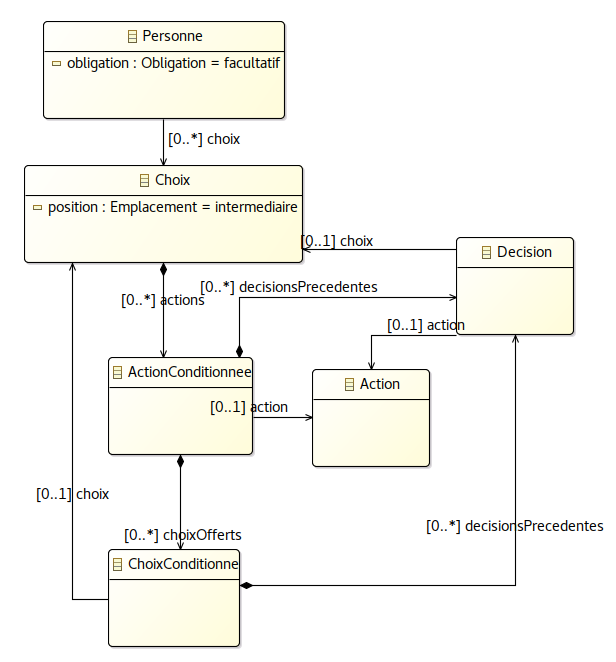
\includegraphics[width=\textwidth]{images/diagram_Interaction}
\newline\newline

\section{Syntaxe Graphique}
Comme pour la syntaxe textuelle, la syntaxe graphique c'est voulue simple. Elle ne permet donc pas de visualiser un jeu dans son ensemble mais seulement les points delicats que sont le territoire et les interactions.
\newline\newline
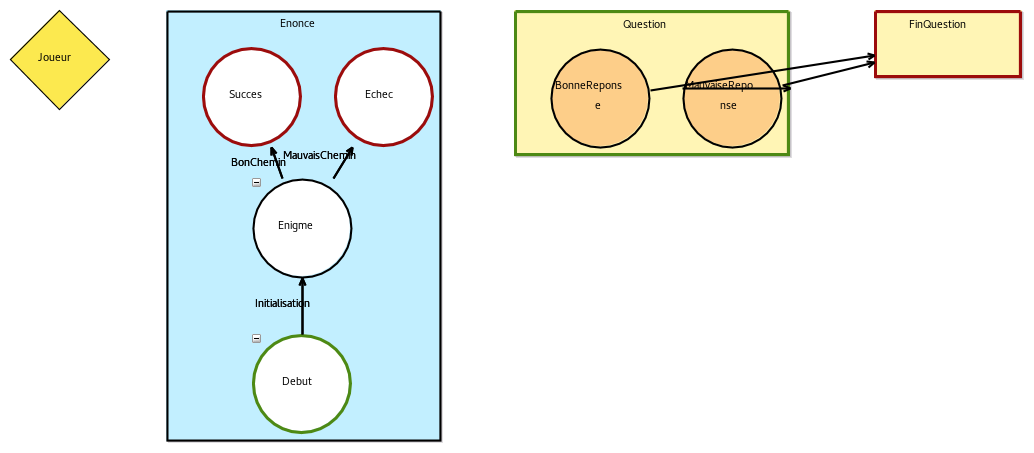
\includegraphics[width=\textwidth]{images/diagram_JeuEnigme}
\newline\newline

\subsection{Point de vue Territoire}
Visualiser les lieux et leurs connections et un point essentiel a la progression du jeu. Les lieux de depart presentent un lisere vert, ceux de fin un rouge et les autres restent noirs. Il est egalement possible de retracte certains lieux afin d'avoir une vue plus complete de l'ensemble. L'utilisateur a egalement la possibilite d'ajouter des lieux ou des chemins directement depuis Sirius.

\subsection{Point de vue Interaction}
Les interactions furent plus techniques a implementer, notamment du fait des multiples conditions sur ces objets. Une interaction se constitue par une suite de choix et d'action. Les actions etant proposee par les choix, elles sont dans ceux -ci, puis reliees aux choix vers lesquelles elles menent.

\section{Verification en PetriNet}
Afin de vérifier les contraintes dynamiques du jeu via l'outil Tina, il a était nécessaire de pouvoir réaliser un réseau de Pétri modélisant le plus précisement possible le jeu.

\subsection{Transformation vers Petrinet}
La transformation vers Petrinet s'est faite via l'outil ATL.\\
Pour contourner un problème d'instanciations non-maitrisées (par exemple, des objets présents dans des conditions se retrouvaient instanciés comme étant des objets réels), nous avons utilisé et couplé les \textit{lazy rules}, les \textit{called rules} et les sections impératives \textit{do}. Ainsi, le modèle est parcouru manuellement et les éléments sont instanciés de façon maitrisée : deux éléments ne seront pas traités de la même façon selon leur utilité réelle déterminée par leur position dans le modèle.\\
De plus, pour représentater les conditions du type \textit{"quantité d'un objet est supérieur / inférieure / égale à $n$"}, nous avons utilisés la combinaison d'arc classiques et d'arcs inhibiteurs découverts lors du parcours de la documentation de l'outil \textit{nd}.\\
Ainsi, bien que la transformation ne soit pas complète (les conditions ne sont pas présentes, la transformation des objets et le fait de poser un objet dans un lieu ne sont pas modélisés), elle permet d'obtenir une bonne représentation du jeu sous forme de réseau de Pétri.
\newline\newline
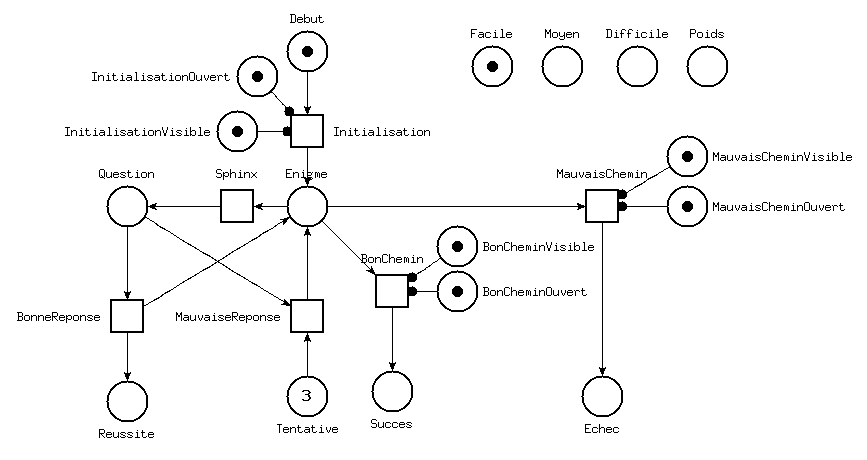
\includegraphics[width=\textwidth]{images/petrinet}
\newline\newline

\subsection{Terminaison du jeu}
Une transformation vers LTL a été créée dans le but de vérifier les contraintes dynamiques. Des templates ont été créés pour faciliter l'écriture de relations logiques.\\
Les contraintes dynamiques actuellement testés sont la terminaison possible du jeu ainsi que l'unicité de la présence dans un lieu (pas de dédoublement de l'explorateur).

\section{Generation de code}
Nous avons décider d'implanter ce jeu en Java.
\subsection{Initialisation du jeu}
Le jeu s'insere directement dans un fichier executable contana t une unique methode main et utilisant des packages codes prealablement. Le code est commente pour permettre a un utilisateur de s'y retrouver plus facilement. Le choix de programmation pris a ete de d'abord declarer l'ensemble des objets, puis de creer les liens entre ces elements. Ceci a evite de devoir utiliser des constructeurs et d'autres accrobaties dans le code Acceleo.

\subsection{Code et Metamodele}
EMF offre des outils pour travailler directement avec un modele en Java par l'intermediaire de Factory. Nous n'avons pas retenu ce choix, le modele genere par Xtext etant trop confu. L'absence d'interface, de classe abstraite ou meme de valeur par defaut (sans passer par les traitements post-generation, complexe et non recommande) nous a conduit a faire un modele complet en Java.\newline
Celui-ci suit les principes Modele-Vue-Controlleur. L'API est utilisable directement pour les utilisateurs aguerris, mais ceux-ci ne disposeront pas des outils de verification.
\subsection{Execution}
Apres compilation du fichier genere par Acceleo, l'utilisateur arrive sur l'interface textuelle presentee page suivante. Celle-ci est sobre et offre a l'utilisateur de multiples propositions. Du fait de la modularite offerte par l'API, les utilisateurs desireux d'avoir une interface plus conviviale et visuelle peuvent laisser libre court a leur imagination pour construite une vue graphique.
\newline\newline
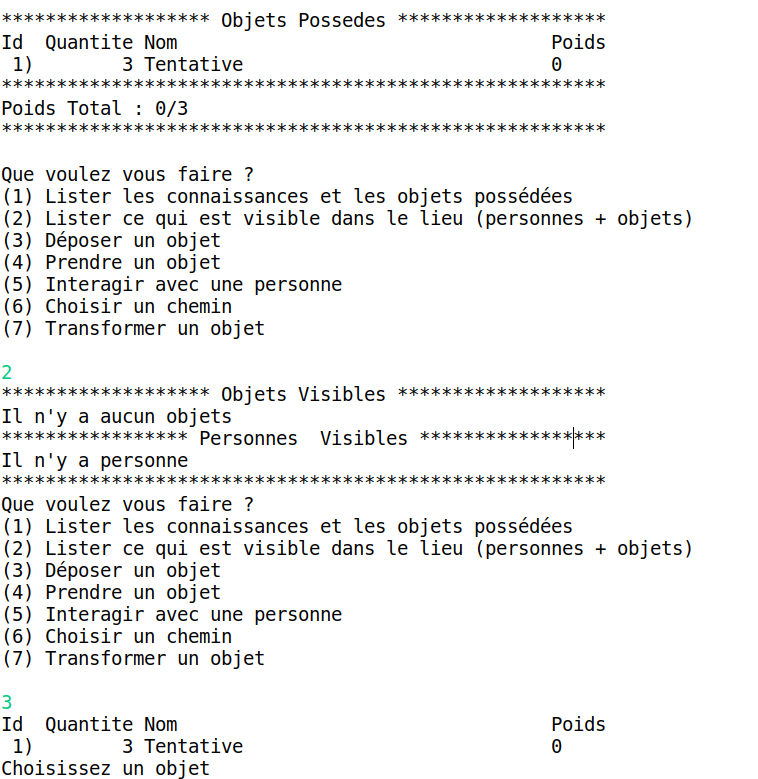
\includegraphics[width=\textwidth]{images/explorateur}
\newline\newline

\newpage
\section*{Conclusion}
Ce projet fut un projet ambitieux. L'objectif principal a ete de rendre une version foncitonnelle fonctionnant sur des exemples simples, notamment celui presente dans ce rapport. Ce dernier a ete atteint a l'aide d'un dialogue permanent entre les membres du groupe. Des changements de modele ont ete opere au fur et a mesure d'une comprehension plus fine du sujet et des caracteristiques techniques qui lui sont associees.\newline
De la generation a l'execution en passant par la verification, nous avons fait face a de multiples difficultes. Documentation rare, interface utilisateur complexe, messages console cryptiques sont les pricipaux problemes auxquels nous avons ete confrontes. L'ide fut cependant plus stable que lors du bilan d'etude, chaque membre travaillant sur une partie specifique et l'integration des differents composants se faisant de maniere plus progressive.\newline
Nous laissons libre cours a votre imagination pour creer les jeux de demain.

\end{document}